\documentclass [pdftex,12pt] {report}
\usepackage [utf8x]{inputenc}
\usepackage [french] {babel}
\usepackage[pdftex]{graphicx}
\usepackage{sidecap}
\usepackage{float}
\usepackage{natbib,hyperref}
\usepackage{indentfirst}
\usepackage[T1]{fontenc} 
\usepackage{amsfonts}
\usepackage{tabularx}
\usepackage{listings}
\usepackage{color}
\usepackage{xcolor}
\usepackage{caption}
\usepackage{textcomp}
\usepackage{adjustbox}

\usepackage{titlesec}
\titleformat{\chapter}[hang]{\Huge\bfseries}{\thechapter\hsp\textcolor{gray75}{|}\hsp}{0pt}{\Huge\bfseries}

\usepackage{hyperref}
\hypersetup{
  backref=true,
  pagebackref=true,
  hyperindex=true,
  breaklinks=true,
  colorlinks=true,
  urlcolor=blue,
  linkcolor=black,
  citecolor=black
}
\definecolor{gray75}{gray}{0.75}
\definecolor{gray}{rgb}{0.4,0.4,0.4}
\definecolor{darkblue}{rgb}{0.0,0.0,0.6}
\definecolor{lightblue}{rgb}{0.0,0.4,0.9}
\definecolor{cyan}{rgb}{0.0,0.6,0.6}
\definecolor{dkgreen}{rgb}{0,0.6,0}
\definecolor{gray}{rgb}{0.5,0.5,0.5}
\definecolor{mauve}{rgb}{0.58,0,0.82}
\definecolor{forestgreen}{RGB}{34,139,34}
\definecolor{orangered}{RGB}{239,134,64}
 
\lstdefinestyle{Java}{
  language=Java,
  basicstyle=\footnotesize\ttfamily,
  numbers=left,
  numberstyle=\tiny\color{gray},
  stepnumber=1,
  numbersep=5pt,
  backgroundcolor=\color{white},
  showspaces=false,
  showstringspaces=false,
  showtabs=false,
  frame=single,
  rulecolor=\color{black},
  tabsize=4,
  breaklines=true,
  breakatwhitespace=false,
  title=\lstname,
  keywordstyle=\color{lightblue},
  commentstyle=\color{dkgreen},
  stringstyle=\color{mauve},
  escapeinside={\%*}{*)},
  keywords=[2]{DATA},
  keywordstyle=[2]\color{red},
  morekeywords={R,View,ViewGroup,TextView,ImageView,ViewHolder}
}

\lstdefinestyle{XML} {
    language=XML,
    frame=single, 
    extendedchars=true, 
    breaklines=true,
    breakatwhitespace=true,
    emph={},
    emphstyle=\color{red},
    basicstyle=\small\ttfamily,
    columns=fullflexible,
    commentstyle=\color{gray}\upshape,
    morestring=[b]",
    morecomment=[s]{<?}{?>},
    morecomment=[s][\color{forestgreen}]{<!--}{-->},
    keywordstyle=\color{orangered},
    stringstyle=\ttfamily\color{black}\normalfont,
    tagstyle=\color{darkblue}\bf,
    morekeywords={attribute,xmlns,version,type,release},
}


\lstdefinestyle{HTML} {
    language=HTML,
    frame=single, 
    extendedchars=true,
    showspaces=false,
    showstringspaces=false,
    showtabs=false,
    breaklines=true,
    breakatwhitespace=true,
    emph={},
    emphstyle=\color{darkblue},
    basicstyle=\tiny\ttfamily,
    columns=fullflexible,
    commentstyle=\color{gray}\upshape,
    morestring=[b]",
    morecomment=[s]{<?}{?>},
    morecomment=[s][\color{dkgreen}]{<!--}{-->},
    keywordstyle=\color{purple},
    stringstyle=\ttfamily\color{black}\normalfont,
    tagstyle=\color{lightblue}\bf,
}

\lstset{language=Java,frame=lines}
\lstset{language=XML,frame=lines}


\def\wl{\par \vspace{\baselineskip}}
\renewcommand{\lstlistingname}{Code}
\newcommand{\HRule}{\rule{\linewidth}{0.5mm}}
\newcommand{\hsp}{\hspace{20pt}}

\begin {document}

\begin{titlepage}
\begin{center}

% Upper part of the page. The '~' is needed because \\
% only works if a paragraph has started.

\includegraphics[width=0.15\textwidth]{./resources/logo}~\\[1cm]

\textsc{\LARGE Université de Bordeaux 1}\\[1.5cm]

\textsc{\Large {Projet de Programmation}}\\[0.5cm]

% Title
\HRule \\[0.4cm]
{ \huge \bfseries Application CampusUB1}\\[0.4cm]

\HRule \\[1.5cm]

% Authors, clients and supervisor
\begin{minipage}{0.4\textwidth}
\begin{flushleft} \large
\emph{Auteurs:} \\
Elyas \textsc{Ben Hadj Yahia}\\
Ryan \textsc{Herbert}\\
Paul \textsc{Maribon-Ferret}\\
Stefan \textsc{Mijatovic}\\
Tatiana \textsc{Rocher}
\end{flushleft}
\end{minipage}
\begin{minipage}{0.4\textwidth}
\begin{flushright} \large
\emph{Clients:} \\
Fabien \textsc{Baldacci}\\
Arnaud \textsc{Casteigts}\\
\emph{\\Encadreur:} \\
Xavier \textsc{Blanc}
\end{flushright}
\end{minipage}

\vfill

% Bottom of the page
{\large \today}

\end{center}
\end{titlepage}
\chapter*{Préface}
Ce document décrit le travail réalisé dans le contexte de notre projet de programmation. Le but de ce projet est de réaliser une application Android permettant d'accéder aux informations pertinentes des différents établissements du campus (Laboratoires, Universités, Ecoles). L'utilisateur choisit les établissements pour lesquels il veut accéder aux informations (dans un premier temps il n'y aura que l'université de Bordeaux 1 et le LaBRI). L'application permet ensuite d'accéder aux annonces d'événements (en offrant la possibilité des les ajouter à l'agenda) et aux annuaires (en offrant la possibilité d'ajouter aux contacts du smpartphone) sélectionnés. \\
\\L'idée est donc de rendre les informations liées aux établissements choisis plus faciles d'accès via un smartphone Android, afin de répondre à un besoin en déplacement, en donnant la possibilité d'enregistrer les informations importantes, et de les intégrer aux applications natives du smartphone, pour permettre une utilité de l'application lorsqu'une connexion Internet n'est pas disponible.
\chapter*{Remerciements}
La réalisation de ce projet n'aurait pas été possible sans l'aide des personnes qui se sont impliqués dans notre travail. Pour cela, nous tenons à remercier:\\\\

Tout d’abord Monsieur Xavier \bsc{Blanc} pour son aide et ses précisions qui nous ont permis de réussir ce projet, sans lesquels nous n'aurions pu aller aussi loin dans l'aboutissement de notre logiciel.\\\\
Monsieur Lionel \bsc{Clément} pour ses conseils au sujet de l’analyse textuelle.\\\\
Nous remercions également nos clients Fabien \bsc{Baldacci} et Arnaud \bsc{Casteigts} pour l’intérêt qu’ils nous ont porté tout au long de notre projet.\\\\
Et finalement Monsieur Philippe \bsc{Narbel} pour ses conseils sur la conduite et le développement de ce projet.

\tableofcontents
\newpage 

\chapter{Etude de l'existant}
\section{Références}


\subsection*{Android Application Development}
L'ouvrage \emph{Android Application Development}~\cite{AndroidBook} est considéré comme l'une des références majeures dans le domaine du développement des applications sur Android.
Il présente notamment l'architecture du système d'opération Android, ainsi que les différentes phases de développement des applications utilisateurs.

\subsection*{Site officiel de la SDK Android}
Le site officiel de la SDK Android~\cite{AndroidSDK} met à disposition des développeurs une panoplie d'outils et de références.
Ce site présente ses divers services, notamment les API d'Android et autres services de Google. On y trouve aussi plusieurs domaines d'application utilisés aujourd'hui qu'on peut intégrer dans notre application.

\subsection*{Article sur les applications mobiles des universités}
Cet article sur les applications mobiles des universités~\cite{Article} décrit les différentes contraintes liées au développement des applications mobiles d'universités. Etant donné que les étudiants sont de plus en plus équipés de smartphones, il devient intéressant de mettre en place une application mobile qui offre divers services utiles et faciles d'accès.


\section{Applications existantes}

\subsection*{uMontréal}
Cette application propriétaire de l'université de Montréal~\cite{uMontreal} met à disposition de ses étudiants de nombreux services, tels que des flux d'actualités, un annuaire, un calendrier, et le plan du campus.

\subsection*{Plateforme Blackboard}
Cette plateforme de développement est utilisée par la majorité des applications campus mobiles aux Etats-Unis~\cite{Blackboard}. On considère par exemple iStandford~\cite{iStanford}, application Android qui présente de nombreux services (internes et externes), dans la même philosophie que l'application uMontréal.

\subsection*{gReader, lecteur de flux RSS}
Ce lecteur de flux RSS~\cite{gReader} offre une interface sobre et pratique pour gérer les abonnements aux flux RSS. Notre développement de l'interface graphique pourra s'inspirer du système des onglets et des toolbars de cette application.

\subsection*{Lecteurs de flux RSS open-source}
Il existe déjà plusieurs lecteurs de flux RSS open-source, tels que Feedgoal~\cite{Feedgoal} et Android-RSS~\cite{Android-RSS}. les deux étant sous licence GNU GPL (v2 et v3, respectivement). On pourra étudier s'il est rentable de reprendre quelques modules, ou de repartir sur notre propre base.


\section{Ressources existantes}

\subsection*{LDAP}
Le protocole LDAP est une ressource potentiellement importante à la conception de notre application, notamment pour la mise en oeuvre de l'annuaire. LDAP signifie Lightweight Directory Access Protocol; c'est donc un protocole conçu uniquement pour les annuaires, et les annuaires du LaBRI et de Bordeaux1 s'avèrent être conformes aux normes LDAP.
Ce sera donc une des technologies importantes à explorer afin de réaliser une réponse robuste au parsage de l'annuaire du LaBRI.\\
Nous nous sommes posés la question de l'accessibilité de l'annuaire venant de l'extérieur, au travers du protocole LDAP; cependant nous allons uniquement utiliser le protocole LDAP pour Bordeaux1 sachant que le serveur LDAP du LaBRI est inaccessible depuis l'extérieur sans passer par un système d'authentification sécurisée.

\subsection*{HTTP/HTML}
Une alternative au protocole LDAP serait d'effectuer des requêtes HTTP, afin de parser des pages HTML. Cette méthode pourrait répondre aux besoins de parser les annuaires dont il en est question, si jamais nous ne pouvons nous reposer sur le LDAP. Le problème posé par cette méthode repose dans la robustesse de la solution. C'est-à-dire qu'un changement de l'implémentation des pages (changement/mise à jour des balises, ou même un changement de forme) pourrait rendre l'application inutilisable. L'utilisation de cette méthode demande énormément de travail de généricité du parsage des pages.
Ceci pose plusieurs problèmes, notamment sur l'imprévisibilité des changements potentielles dans les pages. Il est impossible de prévoir à 100\% les modifications qui pourraient avoir lieu sur les pages, et donc l'application pourrait rapidement devenir inutilisable. Il sera nécessaire de s'inspirer voire de réutiliser certains codes de web crawlers open source afin d'assurer d'avoir une application aussi robuste qu'elle puisse l'être en parsant des pages HTML.


\subsection*{Analyse textuelle}
Au cours de l'implémentation de cette application, nous serons amenés à effectuer de l'analyse textuelle sur des textes afin d'en extraire les informations dont nous avons besoin, par exemple si une date n'est pas au sein d'une balise facilement repérable/exploitable. Il faudra donc tenter d'extraire des dates des textes disponibles. Cela pose plusieurs problèmes:
\begin{itemize}
\renewcommand{\labelitemi}{$\bullet$}
  \item Le texte peut faire référence à un événement passé, simplement à titre informatif, auquel cas, une date extraite n'aurait pas nécessairement de valeur à l'exploitation avec notre application.
  \item Le texte peut contenir plusieurs dates, faisant référence à plusieurs événements passés, présents, ou futurs et il sera donc difficile d'exploiter les informations et de découper le texte en plusieurs événements, ou encore d'extraire la date pertinente à l'événement.
  \item Le texte peut ne contenir aucune date, n'étant simplement qu'une information quelconque.
\end{itemize}
\wl Les événements inscrits dans les flux RSS du site de Bordeaux 1 possèdent une balise \emph{pubDate}, qui devrait faire référence à la date de publication des articles, mais nous avons remarqué que pour la plupart des articles (notamment pour toutes les soutenances), cette date a été modifiée pour correspondre à la date de la soutenance. Cependant, ce n'est pas toujours le cas pour l'horaire. Certains articles possèdent des horaires qui correspondent à celle de l'événement (comme pour les soutenances, par exemple), mais d'autres ont un horaire qui ne correspond pas avec l'horaire de l'événement. Nous avons donc tiré la conclusion que l'horaire correspond parfois à l'horaire de publication de l'article. \\
Il sera donc possible de comparer les dates et horaires extraites par analyse textuelle avec les informations contenues dans la balise \emph{pubDate} afin d'augmenter le taux de réussite de la proposition de date au moment de l'ajout dans l'agenda du smartphone. \\

\begin{lstlisting}[style=XML, caption=Extrait d'un flux RSS de Bordeaux1 (29/01/2013), label=xml1]
<item>
  <title>Trophees du sport</title>
  <link>...</link>
  <description>
	Pour la 3e annee consecutive...
  </description>
  <content:encoded>
    <![CDATA[
      Ils seront recompenses a l occasion des Trophees du sport
      le jeudi 31 janvier 2013 a 18h dans l Atrium...
    ]]>
  </content:encoded>	
  <pubDate>Thu, 31 Jan 2013 15:08:00 +0100</pubDate>
</item>
\end{lstlisting}

\wl Sur cet exemple, l'heure qui apparait dans la balise \emph{pubDate} ne correspond pas à celle de l'événement; il va donc falloir analyser la description pour essayer de trouver l'horaire correspondant (ici 18h). \\

Etant donné ces problèmes, nous devrons surement trouver une approximation au problème, car nous ne pourrons proposer la bonne date à chaque fois qu'un utilisateur souhaite ajouter un élément à son agenda.\\
Il existe plusieurs outils utiles à l'implémentation d'une solution à ces problèmes, notamment des outils de parsing comme JFlex et CUP qui, d'après un livre d'Android~\cite{ProgAndroid} reste une solution possible. Ces outils ressortent pour nous, car leur utilisation nous est déjà familière. Ces outils cumulés avec les informations extraites d'un livre d'analyse textuelle~\cite{analyseTextuelle} sur l'extraction d'information pourront nous permettre de mettre en place une solution efficace à ce problème.\\

\chapter{L'Application CampusUB1}
\section{Aperçu de l'application}

\subsection{Actualités}
Une des fonctionalités principales de l'application est la récupération, l'affichage et l'enregistrement des événements dans le calendrier de l'utilisateur. 
Pour cela, nous prévoyons de récuperer les flux RSS les plus utiles de l'université Bordeaux 1\cite{fluxBDX1}, notamment les flux disponibles sur la page d'accueil du site de l'université (dont les actualités).
En ce qui concerne le site du LaBRI, il n'y a aucun flux RSS et il faudra donc parser directement du code HTML.

\subsection{Annuaire}
Il sera également possible de consulter les annuaires des établissements concernés, afin d'en extraire les informations désirées et les ajouter aux contacts du smartphone.
Afin d'implémenter l'annuaire au sein de notre application Android, il est évident qu'il faut exploiter les annuaires de Bordeaux 1~\cite{AnnuaireBdx1} et du LaBRI. En ce qui concerne le LaBRI, le serveur LDAP n'est pas accessible depuis l'extérieur (sans authentification).Nous devrons donc intégrer l'annuaire à travers des requêtes GET, dans le but de parser les résultats obtenus. Pour le moment ceci semble être la meilleure solution envisageable. L'accès sans authentification au serveur LDAP de l'université de Bordeaux1 nous est permis, ce qui facilitera grandement l'intégration de la recherche dans l'annuaire pour cet établissement, ainsi que la maintenabilité du logiciel.


\subsection{Utilitaires}
\subsubsection{Plan du campus}
Dans un deuxième temps, nous prévoyons de mettre en place un plan du campus, potentiellement intégré à l'application Maps du smartphone.
Ce service permettrait donc à l'utilisateur d'avoir un aperçu plus détaillé du campus en affichant les différents bâtiments et leur noms.
On poura éventuellement aussi afficher les emplacements des différents services dédiés aux étudiants (cafétéria, restaurant universitaire, bibliothèque universitaire, ...).

\subsubsection{Emploi du temps}
Un autre service qui pourrait être très utile en particulier pour les étudiants de Bordeaux1 est l'accès et la sauvegarde locale de leur emplois du temps en fonction de leurs filières, des groupes, et des différentes options suivies. 
Pour cela, nous parserons les fichiers XML des emplois du temps utilisant la plateforme Celcat\cite{EdTxml}, afin de mettre à disposition une copie locale de l'emploi du temps dans l'agenda du smartphone.
\chapter{Analyse des besoins}

Nous allons analyser dans ce chapitre les différents besoins fonctionnels et non-fonctionnels de notre application.\\
Nous allons donc utiliser un système de points pour évaluer la difficulté des tâches. On se basera sur une séquence de Fibonacci arrondie (1, 2, 3, 5, 8, 13, 20, 40, 60, 100), avec 100 reflétant une tâche d'une grande difficulté.\\
Les priorités des besoins sont classées sur cette échelle: optionnel, faible, moyen, important, vital.
\section{Besoins fonctionnels}
\subsection{Fonctionnalités principales}
\subsubsection{Choix des établissements}
Etant donné que l'application présentera des services en commun à plusieurs établissements, l'utilisateur doit pouvoir s'abonner aux établissements de son choix, s'il souhaite accéder à leurs propres informations [Fig.~\ref{fig:01}]. \\

\begin{itemize}
\renewcommand{\labelitemi}{$\bullet$}
\item Priorité: vital
\item Difficulté: 1/100
\item Risques: mise à jour des liens si les adresses des établissements sont modifiées.
\item Validation: s'assurer que les sélections et les modifications des abonnements s'effectuent correctement.
\end{itemize}

\subsubsection{Gestion des actualités}
En accédant au menu des actualités, l'utilisateur disposera d'une interface à travers laquelle il recevra le flux des actualités des établissements auxquels il est abonné. Par défaut il aura alors la possibilité de voir les événements propres aux établissements auxquels il s'est abonné. Il pourra à tout moment changer de catégorie grâce au menu des catégories [Fig.~\ref{fig:04}] depuis la même fenêtre. De plus, il peut choisir entre voir la totalité des actualités des établissements auquels il a souscrit, ou voir uniquement les actualités propres aux établissements qu'il a sélectionné dans les filtres.  [Fig.~\ref{fig:03}]. L'utilisateur doit pouvoir lire l'annonce de ces événements [Fig.~\ref{fig:04}], et doit pouvoir facilement rajouter cet événement au calendrier de son smartphone (Google Calendar). Cette action redirigera l'utilisateur vers le calendrier, dans lequel l'événement sera créé avec les informations récoltées. L'utilisateur pourra donc modifier, valider ou annuler la procédure. \\

\begin{itemize}
\renewcommand{\labelitemi}{$\bullet$}
\item Priorité: vital
\item Difficulté: 40/100
\item Difficultés techniques: extraction des informations pertinentes.
\item Risques: changement de structure du contenu à parser (flux RSS et pages HTML).
\item Validation: assurer l'intégrité des informations extraites.
\end{itemize}

\subsubsection{Accès à l'annuaire}
L'utilisateur doit pouvoir effectuer facilement les tâches suivantes:\\
\begin{itemize}
\renewcommand{\labelitemi}{$\bullet$}
\item Rechercher un contact dans l'annuaire par son nom et/ou prénom.
\item Visualiser les informations d'un contact.
\item Rajouter un contact à la liste des contacts de l'utilisateur (créer un nouveau contact ou éditer existant).
\item Envoyer un mail au contact.
\item Appeler la personne (si un numéro de téléphone est disponible).
\end{itemize}

\wl La recherche de personnes dans l'annuaire se fera en fonction des établissements auxquels l'utilisateur s'est abonné. On pourra donc choisir grâce à un filtre entre rechercher une personne dans l'annuaire propre à un ou plusieurs établissements, ou la rechercher dans tous les annuaires.
Lors de l'ajout d'un contact, l'utilisateur sera redirigé vers la page de création d'un nouveau contact, dans laquelle les champs pertinents seront pré-remplis, en fonction des informations collectées. L'utilisateur pourra donc modifier, valider ou annuler la procédure. \\

\begin{itemize}
\renewcommand{\labelitemi}{$\bullet$}
\item Priorité: vital
\item Difficulté: 40/100
\item Difficultés techniques:
\begin{itemize}
\item Avec LDAP: mise en place du protocole.
\item Sans LDAP: parsage des informations.
\end{itemize} 
\item Risques: changement de structure du contenu à parser.
\item Validation: assurer l'intégrité des informations extraites.
\end{itemize}

\subsubsection{Mises à jour}
Notre application pouvant fonctionner hors connexion, les mises à jour de flux RSS étant de type pull, il est important de proposer les mises à jour sur les flux que nous parsons. Par exemple après une longue période sans connexion nous pourrons sauter sur l'occasion de proposer des mises à jour des flux dès que l'utilisateur ouvre l'application et qu'une connexion internet est disponible. Une autre solution serait de mettre à disposition un bouton \emph{refresh} pour que l'utilisateur puisse effectuer une demande de mise à jour (option préférable pour les personnes ayant un forfait internet limité, ou encore pour l'utilisation à l'étranger). Nous pourrions également proposer une solution intermédiaire, où l'application effectue des mises à jour régulières lorsqu'elle est connectée sur un réseau via le WiFi, mais requiert une demande explicite si le réseau est de type 3G. \\
L'application devra garder en mémoire les derniers éléments téléchargés pendant un mois après la date de l'événement (durée à revoir éventuellement). Ainsi lorsque l'on n'a pas accès à Internet, on pourra accéder à ceux-ci. De plus, lors des mises à jour, on téléchargera uniquement les nouveaux événements. Ceci permettra à l'application d'économiser du temps d'exécution, et potentiellement du crédit à l'utilisateur. \\

\begin{itemize}
\renewcommand{\labelitemi}{$\bullet$}
\item Priorité: important
\item Difficulté: 40/100
\item Risques: mauvaise gestion de la mémoire.
\item Difficultés techniques: éviter de télécharger de nouveau des informations déjà collectées.
\item Validation: vérifier l'intégration des nouvelles informations.
\end{itemize}


\subsection{Fonctionnalités secondaires}
Dans un deuxième temps, nous comptons implémenter quelques options supplémentaires, qui ne rentrent pas dans le cadre du projet initial, mais qu'on estime être assez pratiques et utiles, et permettront de compléter l'application.

\subsubsection{Abonnements et filtrage d'informations}
Après avoir choisi lors du premier démarrage de l'application, les établissements auprès desquels l'utilisateur souhaite s'abonner~[Fig.~\ref{fig:01}], il pourra à tout moment revenir sur son choix à travers le menu des préférences.
Il pourra également en fonction de ses abonnements actifs visualiser la totalité des informations propres à un, plusieurs ou tous les établissements grâce à un outil de filtrage. Cet outil se présente sous la forme d'un menu quasiment identique à celui du choix des abonnements et sera accessible uniquement depuis l'écran d'accueil. \\

\begin{itemize}
\renewcommand{\labelitemi}{$\bullet$}
\item Priorité: optionnel
\item Difficulté: 60/100
\item Difficultés techniques: s'assurer que l'abonnement simultané à un grand nombre d'établissements ait un impact mineur sur la stabilité de l'application.
\item Risques: saturation trop rapide de la mémoire cache.
\item Validation: affichage cohérent des informations liées aux abonnements actifs en un temps raisonnable (de l'ordre de 3 à 4 secondes par établissement).
\end{itemize}

\subsubsection{Emploi du temps}
L'utilisateur étudiant doit pouvoir récupérer son emploi de temps du semestre et l'intégrer à Google Calendar. Il doit pouvoir indiquer sa filière, et éventuellement ses cours et ses groupes. \\

\begin{itemize}
\renewcommand{\labelitemi}{$\bullet$}
\item Priorité: optionnel
\item Difficulté: 60/100
\item Difficultés techniques: extraction des informations en fonction du choix de l'utilisateur.
\item Risques: changement du format de l'emploi du temps.
\item Validation: assurer l'intégrité des données extraites.
\end{itemize}

\subsubsection{Plan du campus}
L'utilisateur pourra naviguer sur le plan du campus en utilisant Google Maps. L'utilisateur disposera des pointeurs vers les bâtiments principaux du campus. \\

\begin{itemize}
\renewcommand{\labelitemi}{$\bullet$}
\item Priorité: optionnel
\item Difficulté: 60/100
\item Difficultés techniques: maîtriser l'API de Google Maps.
\end{itemize}



\section{Besoins non fonctionnels}
\subsection{Besoins de performance}
L'application CampusUB1 est destinée à toute personne étudiant ou travaillant sur le campus de l'université. Elle devra donc être capable de tourner sur les derniers smartphones, tout en restant compatible avec des smartphones plus anciens et donc moins puissants puisque tout étudiant n'a pas forcément les moyens d'aborder un smartphone récent ayant une forte puissance de calcul et une grande quantité de RAM. CampusUB1 ne sera donc pas gourmande en ressources et pourra exécuter ces services de manière assez rapide même sur les smartphones moins performants.\\
Nous testerons l'application sur les appareils suivants: LG Optimus 2X (P990), Sony Xperia S, Samsung Galaxy S3.\\

\begin{itemize}
\renewcommand{\labelitemi}{$\bullet$}
\item Priorité: faible
\item Difficulté: 40/100
\item Difficultés techniques: bonne gestion de l'espace mémoire et de l'actualisation.
\item Risques: implémention complexe et potentiellement longue.
\item Validation: vérification que l'utilisation reste assez fluide et ne consomme pas beaucoup de ressources (à préciser un seuil de consommation de RAM).
\end{itemize}  

\subsection{Besoins de fiabilité}
Etant donné que les différents services mis à disposition par CampusUB1 à ses clients s'avèrent souvent être d'un besoin professionnel, il est essentiel que les données affichées soient cohérentes et en accord avec les données d'origine. Si un chercheur du LaBRI recherche depuis notre application le numéro de la salle où a lieu sa conférence, il a tout intérêt à récupérer une information correcte. CampusUB1 ne peut tout de même pas garantir l'exactitude de toutes les informations données et ne se tient donc pas responsable d'éventuelles erreurs, sachant que l'application se base sur des algorithmes de reconnaissance de textes qui peuvent eux-mêmes être erronés d'origine. Il est évident que certaines questions de sécurité courantes se posent sachant que l'application nécessite une connexion à internet continue, mais vu que CampusUB1 utilise uniquement des données publiques dans les services qu'elle fournit, la question de confidentialité des données ne se pose pas. \\

\begin{itemize}
\renewcommand{\labelitemi}{$\bullet$}
\item Priorité: moyen
\item Difficulté: 60/100
\item Difficultés techniques: fiabilité de l'algorithme d'analyse textuelle pour détecter les dates des événements.
\item Risques: création d'un événement avec des données erronées.
\item Validation: simulation de l'algorithme d'analyse textuelle sur suffisamment de données pour avoir un taux de réussite acceptable (à déterminer).
\end{itemize}  

\subsection{Besoins d'intégrité de données}
CampusUB1 doit accéder à certaines ressources personnelles du client pour pouvoir fonctionner, ce qui pose un problème de protection des données. Le calendrier et le répertoire du client sont les ressources auxquelles l'application est susceptible d'accéder, et on devra s'assurer que toute perte éventuelle de données déjà existantes ne soit pas engendrée par une erreur provenant de l'application. L'erreur humaine étant évidemment toujours possible. Toute modification éventuelle de données privées de l'utilisateur se fera donc impérativement avec son avis. \\

\begin{itemize}
\renewcommand{\labelitemi}{$\bullet$}
\item Priorité: moyen
\item Difficulté: 40/100
\item Risques: perte des informations existantes sur le smartphone.
\item Validation: monitoring du comportement de l'application.
\end{itemize} 


\subsection{Besoins organisationnels}
Etant donné que nous travaillerons sur la plateforme Android, le langage Java nous est imposé vu que l'API Android est fournie en Java.
L'IDE dans lequel nous avons choisi d'implémenter notre application est Eclipse pour de nombreuses questions pratiques. Les développeurs d'Android disposent d'un plugin officiel pour Eclipse, qui facilite le travail du développeur en lui fournissant une panoplie d'outils tels que les différentes perspectives dont celle de débogage qui nous sera très utile. Ce plugin comporte également un émulateur d'appareils Android, ce qui nous permettra de facilement tester l'application sur une multitude d'appareils virtuels. De plus, l'API Android est très documentée et est maintenue fréquemment.
\chapter{Diagrammes de fonctionnement}

\section{Fonctionnalités de l'application}

\begin{figure}[h]
  \center
  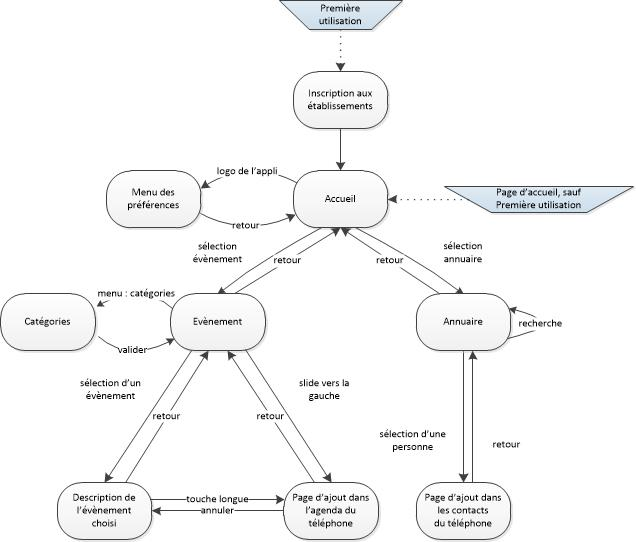
\includegraphics[width=0.92\textwidth]{resources/features1.jpg}
\end{figure}

\newpage

Le diagramme ci-dessus présente toutes les actions réalisables par l'utilisateur et leurs enchaînements.
Lorsque l'utilisateur démarre l'application pour la première fois, il choisit l'établissement auprès duquel il veut s'abonner.
Ce choix est alors retenu, et cette étape est donc omise lors des futurs démarrages de l'application. Une option existera tout de même pour modifier les abonnements si nécessaire. Depuis l'écran d'accueil, l'utilisateur pourra alors accéder aux services de son choix et pourra à tout moment revenir en arrière facilement. \\

\begin{figure}[h]
	\center
	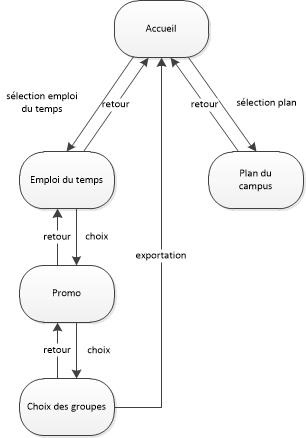
\includegraphics[width=0.6\textwidth]{resources/features2.jpg}
\end{figure}

Le diagramme ci-dessus présente les services offerts pour l'établissement Bordeaux1. Ces services supplémentaires seront accessibles quand l'utilisateur sera abonné à Bordeaux1.

\section{Diagramme des mises à jour}

\begin{figure}[h]
  \center
  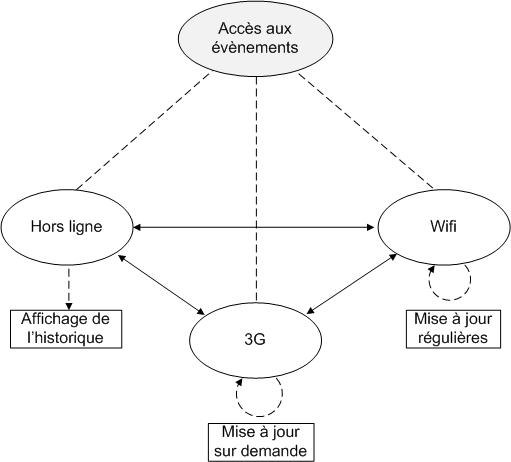
\includegraphics[width=0.6\textwidth]{resources/state_diagram.jpg}
\end{figure}

Le diagramme de mises à jour représente les différents modes de connection dans lesquels on peut se trouver lorsqu'on accède aux événements. Il y a trois modes possibles gérés par le téléphone :\\
\begin{itemize}
\renewcommand{\labelitemi}{$\bullet$}
 \item Hors Ligne : pas d'accès à Internet.
 \item 3G :  accès au réseau de données mobiles (lent).
 \item WiFi : accès à un réseau sans-fil (rapide).
\end{itemize}

\newpage

\section{Diagramme de Gantt}
Le diagramme de Gantt suivant présente une première estimation de la répartition des tâches sur le déroulement du projet. 

\begin{figure}[h]
  \center
  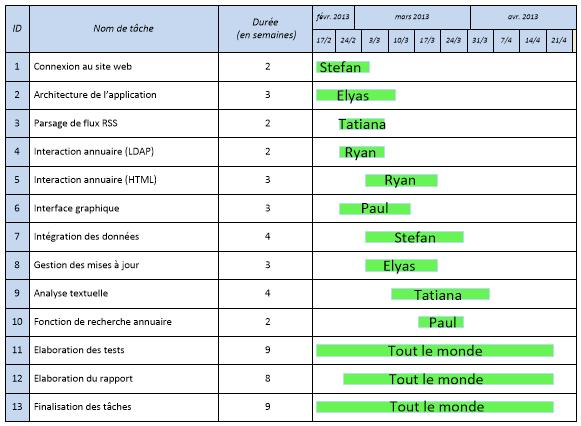
\includegraphics[width=1.0\textwidth]{resources/gantt.jpg}
\end{figure}

Chaque ligne représente une tâche à effectuer, une estimation de sa durée, et son attribution au sein de l'équipe de développement. \\
\chapter{Tests et Validation}
  
  \subsection{Test 01: Choix de l'établissement}
    \begin{enumerate}
    \item Démarrer l'application pour la première fois, un menu vous sera proposé pour effectuer le choix de l'établissement~[Fig.~\ref{fig:01}].
    \item Sélectionnez les établissements auxquels vous voulez vous abonner (on peut annuler pour quitter l'application).
    \end{enumerate}

    \underline{Résultat attendu}: Vous serez redirigé vers le menu principal de l'application.

  \subsection{Test 02: Maintien du choix des établissements}
    \begin{enumerate}
    \item Quittez l'application, et redémarrez-la.
    \end{enumerate}

    \underline{Résultat attendu}: L'application aura sauvegardé vos abonnements, et vous redirigera sur la page d'accueil de l'application.

  \subsection{Test 03: Evénements}
    \begin{enumerate}
    \item Une fois les abonnements configurés, sélectionner le menu des événements dans le menu principal~[Fig.~\ref{fig:02}].
    \end{enumerate}

    \underline{Résultats attendus}:
    \begin{itemize}
    \item Si l'application est connectée à Internet: Les événements de tous les établissements auxquels l'application est abonnée sont affichés~[Fig.~\ref{fig:04}].
    \item Sinon: Les événements ayant déjà été téléchargés sont affichés.
    \end{itemize}

  \subsection{Test 04: Validité des informations extraites d'un évenement}
    \begin{enumerate}
    \item Depuis l'accueil, appuyer sur Evénements.
    \item Naviguer dans la liste des événements.
    \item Appuyer sur un événement afin d'afficher la vue détaillée~[Fig.~\ref{fig:06}].
    \item Appuyer sur le bouton \emph{Plus}, ou bien \emph{Menu->Ajouter}.
    \end{enumerate}

    \underline{Résultat attendu}: Redirection vers la page de création d'événements de Google Calendar, avec les informations correspondantes à celles contenues dans l'événement.

  \subsection{Test 05: Ajout d'un événement au smartphone}
    \begin{enumerate}
    \item Effectuer le Test 04.
    \item Valider l'ajout de l'événement.
    \end{enumerate}

    \underline{Résultat attendu}: L'événement sera ajouté à l'agenda du téléphone.


  \subsection{Test 06: Annuaire}
    \begin{enumerate}
    \item Sélectionner \emph{Annuaire} dans le menu d'accueil.
    \end{enumerate}

    \underline{Résultats attendus}:
    \begin{itemize}
    \item Si l'application est connectée à Internet: on arrive sur l'écran de la~figure~\ref{fig:07}.
    \item Sinon : un toast nous prévient qu'on est déconnecté.
    \end{itemize}

  \subsection{Test 07: Rechercher dans l'Annuaire}
    \begin{enumerate}
    \item Accéder à l'annuaire à partir du menu principal.
    \item Effectuer une recherche~[Fig.~\ref{fig:08}], cela affichera tous les contacts qui correspondent à la recherche, parmis les établissements auxquels l'application est abonnée.
    \end{enumerate}

    \underline{Résultat attendu}: Les résultats se réduisent à ceux qui correspondent à la recherche.

  \subsection{Test 08: Validité des informations extraites}
    \begin{enumerate}
    \item Depuis l'accueil appuyer sur \emph{Annuaire}
    \item Effectuer une recherche de contact.
    \item Effectuer une touche longue sur un contact.
    \item Sélectionner \emph{Ajouter un nouveau contact}.
    \end{enumerate}

    \underline{Résultat attendu}: Redirection vers la page de création de contact, pré-remplie avec les informations correspondantes à celles contenues dans le résultat de recherche.

  \subsection{Test 09: Ajout d'un contact au téléphone}
    \begin{enumerate}
    \item Effectuer le Test 08.
    \item Valider l'ajout/l'édition du contact
    \end{enumerate}

    \underline{Résultat attendu}: Les informations se trouvent dans les contacts du téléphone.

  \subsection{Test 10: Appeler un contact}
    \begin{enumerate}
    \item Depuis le menu d'accueil, appuyer sur \emph{Annuaire}.
    \item Sélectionner un contact possédant un numéro de téléphone.
    \item Effectuer une touche longue sur un contact.
    \item Sélectionner \emph{Appeler}
    \end{enumerate}

    \underline{Résultat attendu}: L'application démarrera un appel vers ce contact.

  \subsection{Test 11: Envoyer un mail à un contact}
    \begin{enumerate}
    \item Depuis le menu d'accueil appuyer sur \emph{Annuaire}.
    \item Sélectionner un contact possédant une adresse mail.
    \item Effectuer une touche longue sur un contact.
    \item Sélectionner \emph{Envoyer un email}
    \end{enumerate}

    \underline{Résultat attendu}: L'application ouvre le gestionnaire d'email du smartphone avec le destinataire rempli avec l'adresse email du contact.

  \subsection{Test 12: Exporter un emploi du temps}
    \begin{enumerate}
    \item S'abonner à un établissement permettant l'exportation d'emplois du temps (ex: Bordeaux1).
    \item Depuis le menu d'accueil, appuyer sur \emph{Export emploi du temps}.
    \item Sélectionner un niveau d'études~[Fig.~\ref{fig:09}].
    \item Sélectionner une filière et un groupe~[Fig.~\ref{fig:10}].
    \item Appuyer sur \emph{Exporter}
    \end{enumerate}

    \underline{Résultat attendu}:
    \begin{itemize}
    \item Si l'application est connectée à Internet: l'emploi du temps choisi est intégré au calendrier du smartphone.
    \item Sinon: Le test échoue dès la première étape, un toast apparait pour indiquer qu'une connexion est nécessaire.
    \end{itemize}

  \subsection{Test 13: Afficher le plan du campus de Bordeaux1}
    \begin{enumerate}
    \item S'abonner à un établissement permettant ayant un plan de campus (ex: Bordeaux1).
    \item Sélectionner \emph{Plan du Campus} dans le menu d'accueil.
    \end{enumerate}

    \underline{Résultat attendu}:
    \begin{itemize}
    \item Si le GPS est activé: ouvre l'application Google Maps centrée sur le campus de Bordeaux1.
    \item Sinon: Affiche une image du plan du campus de Bordeaux1.
    \end{itemize}

\chapter{Architecture}
\section{Aperçu de l'architecture}

\begin{figure}[h]
  \label{fig:architecture}
  \center
  \setlength\fboxsep{5pt}
  \setlength\fboxrule{0.5pt}
  \fbox{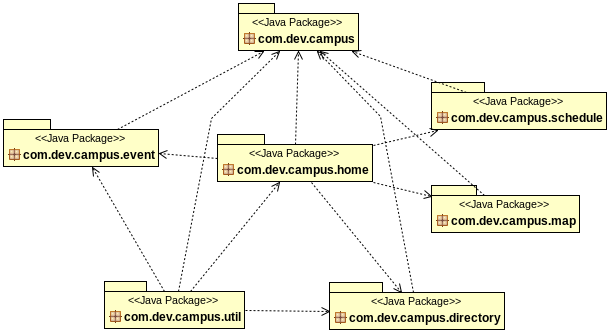
\includegraphics[width=0.9\textwidth]{resources/architecture.png}}
\end{figure}

L'application est organisée en plusieurs packages, chacun définissant des services différents. On distingue les modules les plus importants: Settings, Directory, et Events.

\newpage
\subsection{Settings}

\begin{figure}[h!]
  \label{fig:preferences_mod}
  \center
  \setlength\fboxsep{5pt}
  \setlength\fboxrule{0.5pt}
  \fbox{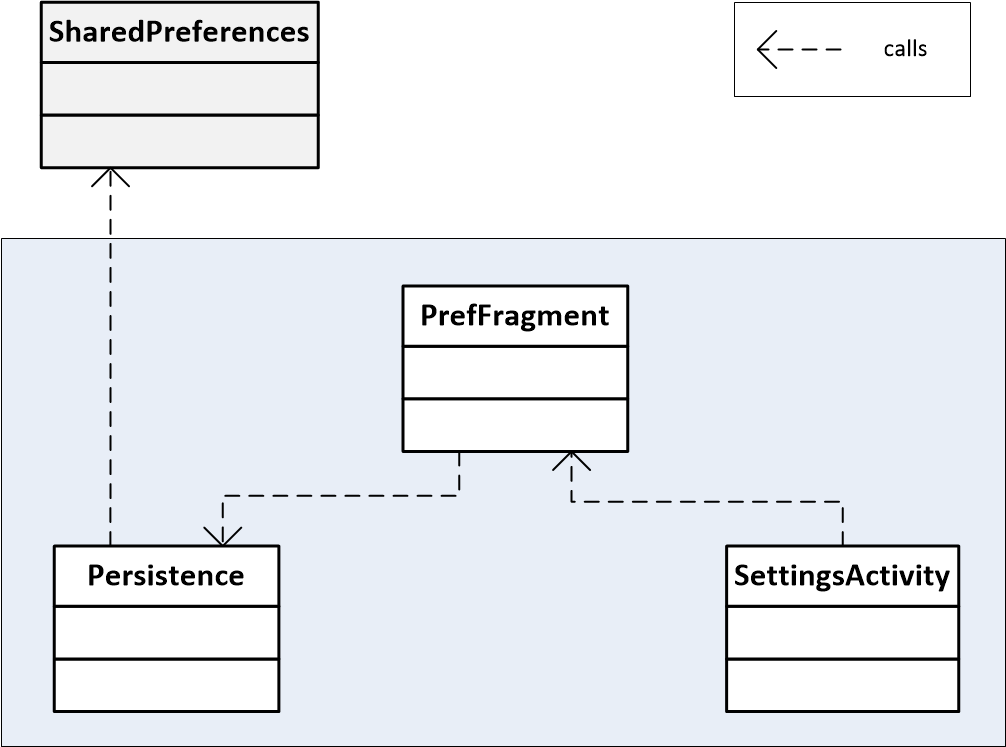
\includegraphics[width=0.9\textwidth]{resources/preferences_mod.png}}
\end{figure}

Ce module s'occupe de la gestion des préférences de l'utilisateur. Toutes les opérations de lecture/écriture des préférences sont effectuées à travers ce module, notamment la gestion des abonnements et des filtres.

\newpage
\subsection{Directory}

\begin{figure}[h!]
  \label{fig:contacts_mod}
  \center
  \setlength\fboxsep{5pt}
  \setlength\fboxrule{0.5pt}
  \fbox{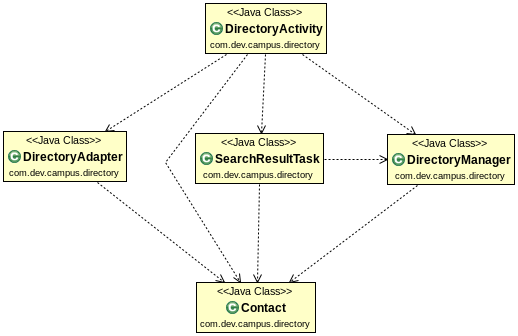
\includegraphics[width=0.9\textwidth]{resources/contacts_mod.png}}
\end{figure}

Ce module s'occupe de la gestion de l'annuaire. Il est responsable des services suivants:
\begin{itemize}
\renewcommand{\labelitemi}{$\bullet$}
\item Parsage des réponses LDAP / pages HTML.
\item Stockage et sauvegarde des données.
\item Affichage graphique des contacts de l'annuaire.
\end{itemize}

\newpage
\subsection{Events}

\begin{figure}[h!]
  \label{fig:events_mod}
  \center
  \setlength\fboxsep{5pt}
  \setlength\fboxrule{0.5pt}
  \fbox{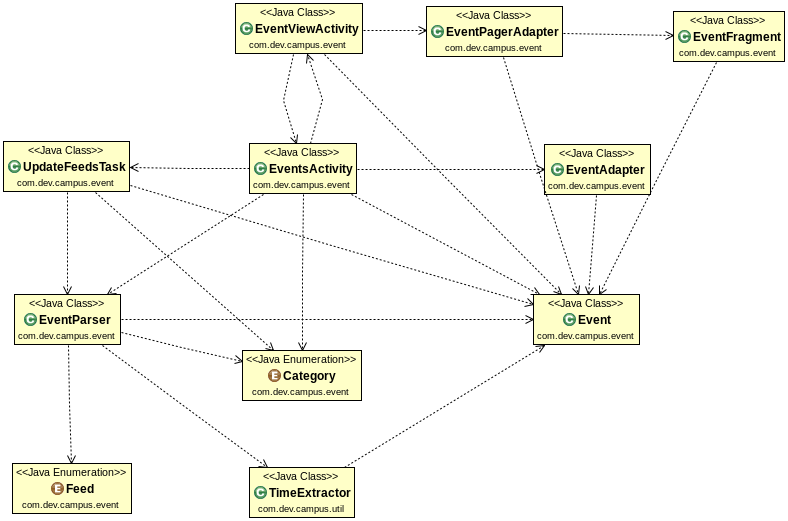
\includegraphics[width=1.0\textwidth]{resources/events_mod.png}}
\end{figure}

Ce module s'occupe de la gestion des événements. Il est responsable des services suivants:
\begin{itemize}
\renewcommand{\labelitemi}{$\bullet$}
\item Parsage des flux RSS / pages HTML.
\item Stockage et sauvegarde des données.
\item Affichage graphique des événements.
\end{itemize}

\chapter{Patterns et descriptions techniques}

\section{Librairies externes utilisées}

Afin de pouvoir implémenter une partie de nos fonctionnalités principales et d'optimiser l'expérience utilisateur de l'application, nous avons eu à faire recours à plusieurs bibliothèques externes. Pour cela, il a avant tout fallu se documenter à propos des bibliothèques existantes et avoir des avis sur celles-ci afin de s'assurer qu'elles soient bien stables, à jour, et qu'elles fournissent tous les services qui nous sont nécessaires.\\

L'application utilise cinq bibliothèques externes: \\

\begin{itemize}
\renewcommand{\labelitemi}{$\bullet$}
\item \textbf{UnboundID LDAP SDK}: indispensable pour la connexion aux serveurs utilisant le protocole LDAP étant donné que la SDK de Java ne fournit aucun outil équivalent. On avait également encore le choix avec \textit{JNDI LDAP} et \textit{Spring LDAP} qui sont deux bibliothèques LDAP connues mais beaucoup plus complexes à utiliser et obsolètes. \\
\item \textbf{Jsoup}: la bibliothèque de référence pour l'analyse textuelle de textes HTML. Elle sert a parser les événements ainsi que l'annuaire du LaBRI. \\
\item \textbf{Google Play Services lib}: librairie nécessaire pour utiliser les services de Google Maps et donc implémenter les services affectant le plan du campus. \\
\item \textbf{Sliding menu lib}: sert à améliorer l'esthétique et l'expérience utilisateur au sein du service qui affiche les événements. Permet de rajouter une barre latérale qui sert à basculer entre les différentes catégories d'événements à tout moment en faisant un simple geste de glissement avec le doigt. \\
\item \textbf{Robotium}: bibliothèque spécifique à la plateforme Android qui nous a été utile durant la phase finale du projet afin d'effectuer des tests en boîte noire pour notre interface graphique. 
\end{itemize}

\section{Extraction des dates}
L’extraction des dates se fait a l’aide d’expressions régulières que l’on applique au contenu des événements. Nous détectons les dates “standalone” pour marquer le début des événements, mais aussi les intervalles de dates afin de pouvoir préciser une durée d’événement lorsque l’utilisateur se décide à ajouter l’événement au calendrier de son téléphone.

\section{Recyclage de vues dans ListView}
Android fournit des outils pour la gestion des listes graphiques, notamment ListView couplée avec l’interface ListAdapter.\\
ListView est conçue pour être extensible et performante, ce qui signifie:

\begin{enumerate}
\item ListView va essayer d’effectuer des inflations de vues aussi peu que possible.
\item ListView ne va dessiner et disposer ses fils que quand ils sont visibles sur l’écran (ou sur le point de l'être).
\end{enumerate}

Le point 1 se justifie par le fait que les opérations d’inflation de layout sont coûteuses (de l’ordre de 1kB de RAM par vue). Ce problème est résolu par le recyclage des vues non visibles, qu’on appelle \emph{ScrapView}. Cela signifie qu’on peut utiliser des vues recyclées et les mettre à jour, au lieu de faire des inflations de vues pour chaque rangée.

Afin d’implémenter le point 2, ListView utilise un recycleur de vues qui déplacera les vues actives dans une pool recyclable quand elles sortent de l’écran. Ainsi, //TODO

\begin{figure}[h]
  \center
  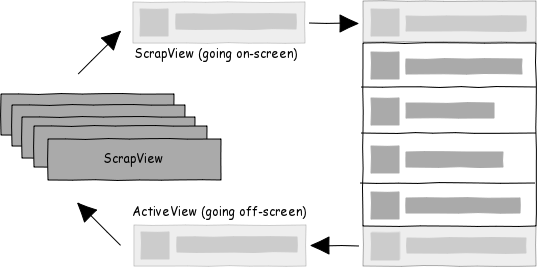
\includegraphics[width=0.92\textwidth]{resources/listview_recycling.png}
\end{figure}

A chaque fois que ListView a besoin d’afficher une nouvelle ligne sur l’écran, elle appelle la méthode \emph{getView()} depuis son adapter.

\begin{adjustbox}{minipage=1.12\textwidth,margin=0pt \smallskipamount,center}
\begin{lstlisting}[style=Java, label=listview1]
public View getView(int position, View convertView, ViewGroup parent)
\end{lstlisting}
\end{adjustbox}

L’argument \emph{convertView} est essentiellement une vue recyclée (\emph{ScrapView}), comme indiqué précédemment. Quand il aura une valeur non nulle, il faudra donc en profiter pour simplement mettre à jour les données au lieu de faire une nouvelle inflation de layout.

\begin{adjustbox}{minipage=1.14\textwidth,margin=0pt \smallskipamount,center}
\begin{lstlisting}[style=Java, label=listview2]
public View getView(int position, View convertView, ViewGroup parent){ 
	View item = mInflater.inflate(R.layout.list_item_icon_text, null);
	((TextView) item.findViewById(R.id.text)).setText(DATA[position]); 
	((ImageView) item.findViewById(R.id.icon)).setImageBitmap(mIcon);
	return item; 
}
\end{lstlisting}
\end{adjustbox}

\chapter{Profiling}
En entammant la phase de test de notre application, nous avons tout de suite décidé d'attribuer à une personne de l'équipe les tâches de profiling qui sont cruciales afin d'optimiser au mieux les performances de l'application. 
Le plugin Android intégré à l'environnement de développement Eclipse nous fournit de base une panoplie d'outils utiles pour réaliser ces tâches. Ces outils se trouvent au sein de la perspective \emph{DDMS} (Dalvik Debug Monitor Server) de Eclipse.
Parmi ces outils, nous nous sommes essentiellement servi de quatre d’entre eux pour obtenir des informations sur le déroulement de notre application: Systrace, Method Profiling, Thread Tracking, et Network Statistics.
 
\section{Systrace}
L'outil Systrace trace une frise pendant une période donnée de marche de notre application, et nous montre les temps d'exécution de nos différents processus ainsi que des processus du système Android. De plus, il nous indique si l'utilisation du CPU durant l'exécution de ces tâches est plus ou moins intense. Dans notre cas, l'utilisation de cet outil nous a servi à déterminer et comparer les temps d'exécution de nos principaux services qui s'occupent de récupérer des donnés puis de les afficher (récupération et affichage des événements, recherche dans l'annuaire de personnes puis affichage de la liste des personnes trouvées...). En effet, nos temps d'exécution ainsi que d'affichage devaient respecter les temps évoqués dans le cahier des charges fourni aux clients. \\
Lors de la première capture du chargement des événements grâce à Systrace, nous avons pu constater que les performances de l'application pouvaient être optimisés lors de l'affichage des éléments qui est assez irrégulier.(Voir figure 8.1)

\begin{figure}[h!]
  \label{fig:systrace_non_optim}
  \center
  \setlength\fboxsep{5pt}
  \setlength\fboxrule{0.5pt}
  \fbox{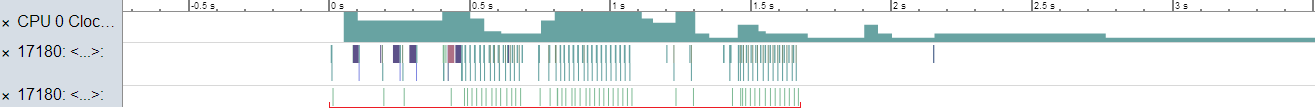
\includegraphics[width=0.9\textwidth]{resources/profiling/systrace/ub1events_non_optim.png}}
  \caption{Récupération et affichage des événements de l'université de Bordeaux 1 avant optimisation}
\end{figure}

L'élément qui nous a permis d'effectuer cette amélioration se trouve au niveau du \textit{layout} qui affiche la liste des événements récupérés. Après s'être renseigné au sein de la documentation Android, nous avons appris que la  modification de l'attribut booléen \textit{android:baselineAligned} à \textit{false} au sein du \textit{layout} permet de gagner en performances en libérant l'application de la charge supplémentaire qu'elle avait à devoir aligner les \textit{baselines} des éléments fils (Voir figure 8.2).

\begin{figure}[h!]
  \label{fig:systrace_optim}
  \center
  \setlength\fboxsep{5pt}
  \setlength\fboxrule{0.5pt}
  \fbox{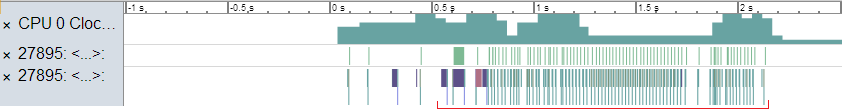
\includegraphics[width=0.9\textwidth]{resources/profiling/systrace/ub1events_optim.png}}
  \caption{Récupération et affichage des événements de l'université de Bordeaux 1 après optimisation}
\end{figure}

Comme on peut le voir sur l'enregistrement précédent, l'affichage des éléments se fait maintenant de manière nettement plus régulière que lors du premier enregistrement. L'optimisation de l'interface graphique a également permis une optimisation globale des performances de l'application puisque le temps d'exécution global(parsing et affichage) diminue automatiquement. 

\section{Method profiling}
Voici un tableau récapitulatif des temps d’exécution de nos fonctionnalités principales sur différents smartphones. Pour chacune d'elles, nous avons effectué des enregistrements qui montrent les temps d'exécution approximatifs des méthodes qui réalisent ces services. Les temps affichés correspondent donc au temps total d'exécution de nos threads appelés\textit{AsyncTask} qui représentent les tâches lourdes exécutes en arrière plan. Ces résultats sont approximatifs et peuvent varier étant donné que le temps d’exécution des méthodes dépend surtout de la fluidité de la connexion Internet utilisée.\\

\begin{figure}[h!]
  \label{fig:benchmark}
  \center
  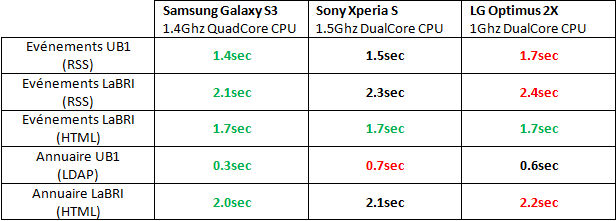
\includegraphics[width=0.9\textwidth]{resources/benchmark.png}
\end{figure}

Le temps obtenu pour le chargement des événements de l'Université de Bordeaux 1 est d'environ de 1.5 secondes(cf. figure~\ref{fig:method_prof1}), ce qui respecte largement les trois à quatre secondes indiquées dans le cahier des charges. Cela est du au fait que les événements de l'Université de Bordeaux 1 correspondent uniquement à des flux RSS à récupérer, ce qui représente une tâche peu couteuse et qui s'exécute relativement vite.
En ce qui concerne l'abonnement au LaBRI, les événements sont récupérés de deux manières distinctes en fonction de la catégorie demandée. Ils pourront donc être récupérés soit via les flux RSS soit en parsant directement les pages HTML du site web. Cela explique alors le temps plus long (2.1 secondes) nécessaire au chargement des actualités du LaBRI sachant que le parsing de pages HTML est plus couteux qu'une simple récupération de flux RSS étant donné qu'il y a une grande quantité d'événements à parcourir, dont certains datant d'il y a plusieurs années. Dans tous les cas, on respecte toujours largement le temps évoqué dans le cahier des charges avec un temps d'exécution tout à fait correct. (cf. figure~\ref{fig:method_prof2})\\\\
 

La recherche dans l'annuaire de l'Université de Bordeaux 1 s'effectue de manière quasiment instantanée: 0.3 sec pour une première recherche (cf. figure~\ref{fig:method_prof3}). Cela est du au fait qu'on utilise une authentification auprès de l'annuaire de Bordeaux 1 en utilisant le protocole LDAP qui nous permet d'avoir une réponse rapide de la part du serveur. De plus, et étant donné que nous sommes limités par le serveur quand au nombre de résultats retournés suite à une requête (dix résultats maximum), l'utilisation du système \emph{Simple paged result control} nous permet de demander au serveur une page de résultats contenant donc dix contacts au maximum. Cela nous évite donc de surcharger le serveur et nous permet d'avoir sa réponse plus rapidement. L'utilisation d'un \emph{Connection pool} nous permet également de maintenir plusieurs connexions actives simultanément auprès du serveur LDAP, et donc de diminuer le temps de retour des requêtes lors de recherches successives dans l'annuaire. (moins de 0.2 secondes lors de la deuxième requête). Il est à noter que le temps de réponse peut varier en fonction de l'état du serveur LDAP de Bordeaux 1 qui peut être plus ou moins occupé à un moment précis.\\\\

Etant donné que les contacts du LaBRI sont récupérés à l'aide du parsing HTML, il est évident qu'ils prennent plus de temps à être parcourus que ceux provenant de l'Université de Bordeaux 1 (cf. figure~\ref{fig:method_prof4}) En effet lorsqu'on effectue une requête auprès d'un serveur LDAP, on recherche uniquement la tranche de l'annuaire correspondant à la recherche effectuée, alors que dans le cas du parsing de l'annuaire du LaBRI, on parcourt la totalité des contacts présents sur la page HTML et on renvoie uniquement ceux correspondants aux critères de recherche. Cela explique donc les temps supérieurs de la recherche de contacts lorsqu'on est abonné au LaBRI (environ 2 secondes) qui découlent de la complexité accrue de l'algorithme d'analyse textuelle effectué lors de chaque requête. Cependant, ces deux secondes représentent un temps plus que correct qui est toujours suffisamment petit pour ne pas avoir d'impact sur l'expérience utilisateur.


\section{Thread tracking}
Grâce à cet outil, nous avons pu observer en temps réel l’activité des threads exécutés par notre application. Après avoir analysé plus précisément leur comportement pour chacun des services proposés, nous avons pu remarquer un défaut dans notre implémentation de la recherche dans l’annuaire de l’université de Bordeaux 1. A chaque fois que nous effectuons une recherche auprès du serveur LDAP, nous nous connections de nouveau auprès du serveur sans réutiliser la connexion précédemment établie. Nous pouvions alors constater (voir code et figure ci-dessous) qu’à chaque fois qu’une nouvelle recherche était effectuée (représentée par le thread AsyncTask), un nouveau thread ConnectionReader  était crée pour se ré-authentifier inutilement au serveur LDAP.

\begin{figure}[h!]
  \label{fig:without_pool_code}
  \center
  \setlength\fboxsep{5pt}
  \setlength\fboxrule{0.5pt}
  \fbox{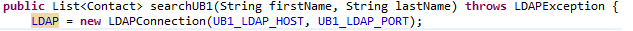
\includegraphics[width=0.9\textwidth]{resources/profiling/code_screenshots/code_without_pool.png}}
\end{figure}

\begin{figure}[h!]
  \label{fig:without_pool}
  \center
  \setlength\fboxsep{5pt}
  \setlength\fboxrule{0.5pt}
  \fbox{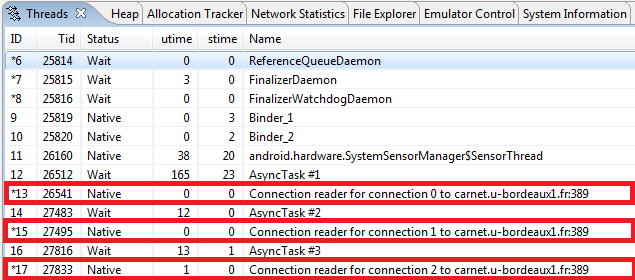
\includegraphics[width=0.9\textwidth]{resources/profiling/code_screenshots/threads_without_pool.png}}
\end{figure}

Cela nous a donc permis de rectifier ce problème en faisant en sorte de réutiliser l’authentification déjà existante, mais également d’apporter une optimisation en se servant de «pools de connexion» qui servent à maintenir plusieurs connexions établies auprès du serveur (10 au maximum),  et qui peuvent être réutilisées par plusieurs threads.\\
On se retrouve donc à présent dans une situation où lorsqu’on effectue plusieurs recherches consécutives dans l’annuaire de Bordeaux 1, un seul thread ConnectionReader est créé pour établir la connexion, et les AsyncTask correspondants aux recherches réutilisent la connexion établie au préalable (voir code et figure ci-dessous).

\begin{figure}[h!]
  \label{fig:with_pool_code}
  \center
  \setlength\fboxsep{5pt}
  \setlength\fboxrule{0.5pt}
  \fbox{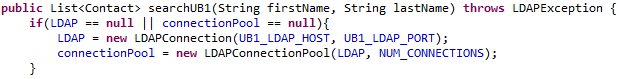
\includegraphics[width=0.9\textwidth]{resources/profiling/code_screenshots/code_with_pool.png}}
\end{figure}

\begin{figure}[h!]
  \label{fig:with_pool}
  \center
  \setlength\fboxsep{5pt}
  \setlength\fboxrule{0.5pt}
  \fbox{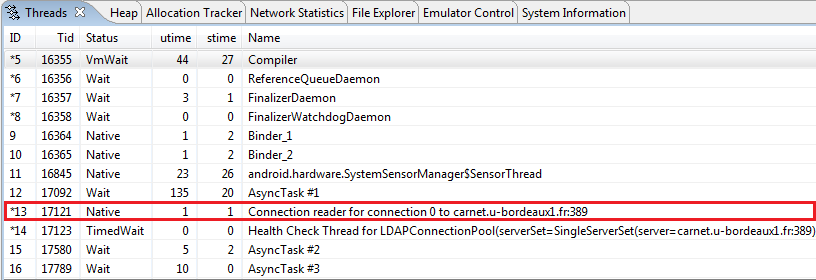
\includegraphics[width=0.9\textwidth]{resources/profiling/code_screenshots/threads_with_pool.png}}
\end{figure}

\newpage

\section{Network statistics}
L’outil d’analyse de paquets transitant sur le réseau à également été une statistique intéressante qui nous a permis de déterminer que notre application n’est pas en état de saturer un réseau, et de vérifier qu’elle n’est pas trop gourmande vis à vis du trafic de données.\\
D’après les analyses effectuées (Voir figure 8.3), lorsqu’on est connecté en Wi-Fi à un réseau haut débit (ADSL dans le cas de notre test), et qu’on récupère la totalité des événements (abonné à l'université de Bordeaux 1 et au LaBRI), le réseau est utilisé pendant environ 7 secondes et de manière discontinue ce qui l’empêche d’être saturé. Durant ces quelques secondes, l’application reçoit en moyenne 57 Ko de données pour afficher la totalité des informations nécessaires, ce qui est relativement une petite quantité de données qui ne pose aucun problème pour être récupérée même sur des connexions à plus faible débit tels que les réseaux mobiles (3G, EDGE, GPRS). 

\begin{figure}[h!]
  \label{fig:network_statistics_events}
  \center
  \setlength\fboxsep{5pt}
  \setlength\fboxrule{0.5pt}
  \fbox{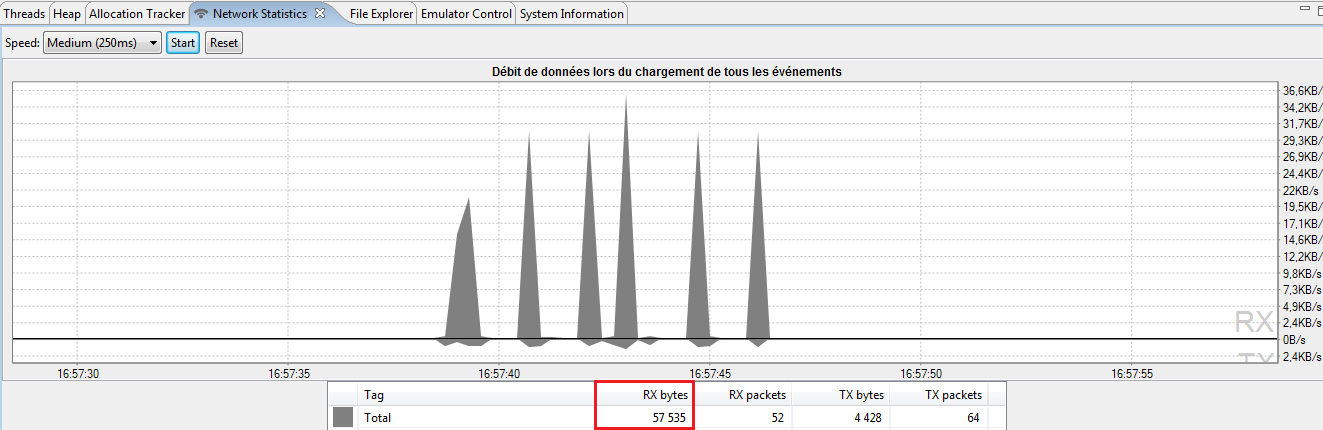
\includegraphics[width=0.9\textwidth]{resources/profiling/network_statistics/events.png}}
  \caption{Utilisation du réseau lors de la récupération de la totalité des événements du LaBRI et de Bordeaux 1}
\end{figure}

Il en est de même pour l’utilisation de l’annuaire (Voir figure 8.4) où la quantité de données à récupérer est encore plus faible (environ 26 Ko) et varie de façon minimale en fonction de la recherche effectuée. 

\begin{figure}[h!]
  \label{fig:network_statistics_directory}
  \center
  \setlength\fboxsep{5pt}
  \setlength\fboxrule{0.5pt}
  \fbox{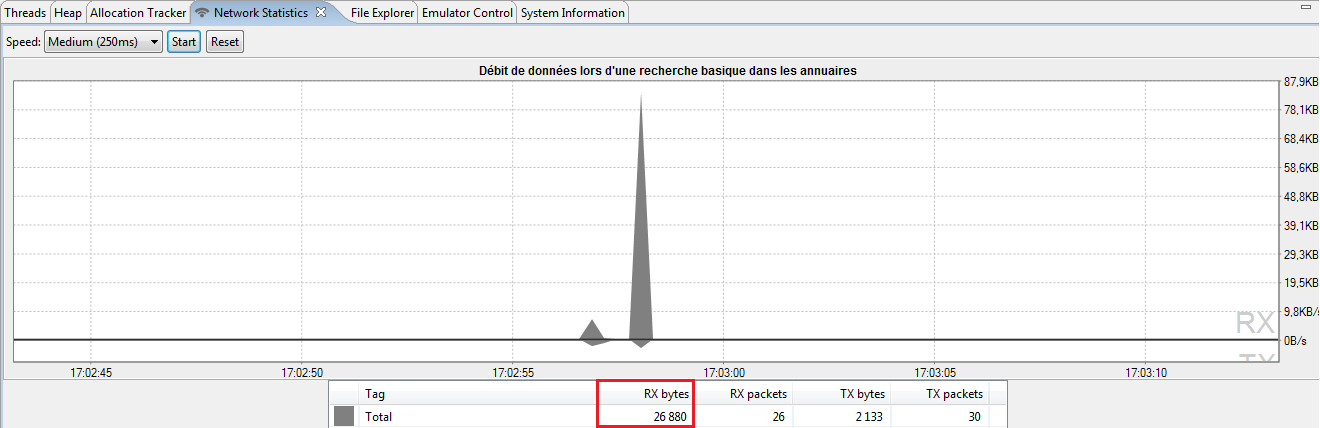
\includegraphics[width=0.9\textwidth]{resources/profiling/network_statistics/directory.png}}
  \caption{Utilisation du réseau lors d'une recherche basique dans les deux annuaires à la fois}
\end{figure}

Ces éléments prouvent que notre application est apte à tourner de manière optimale sur des supports mobiles divers, utilisés en extérieur lorsqu’une connexion haut débit ne se trouve pas forcément à proximité.
\chapter{Exemple d'utilisation}

Les images suivantes représentent un premier aperçu de l'interface graphique de l'application. Nous imaginons donc un scénario d'utilisation qui montre le déroulement d'un usage typique.

\begin{figure}
  \begin{minipage}[t]{8cm}
    \centering
    
\includegraphics[width=0.8\textwidth]{resources/ui_preview/01}
    \caption{Lors du premier lancement de l'application, l'utilisateur doit sélectionner ses établissements. Une fois ses choix effectués, il sont enregistrés et ne seront plus demandés. Les établissements sont modifiables via les préférences.}
    \label{fig:01}
  \end{minipage}
  \hspace{+20pt}
  \begin{minipage}[t]{8cm}
    \centering
    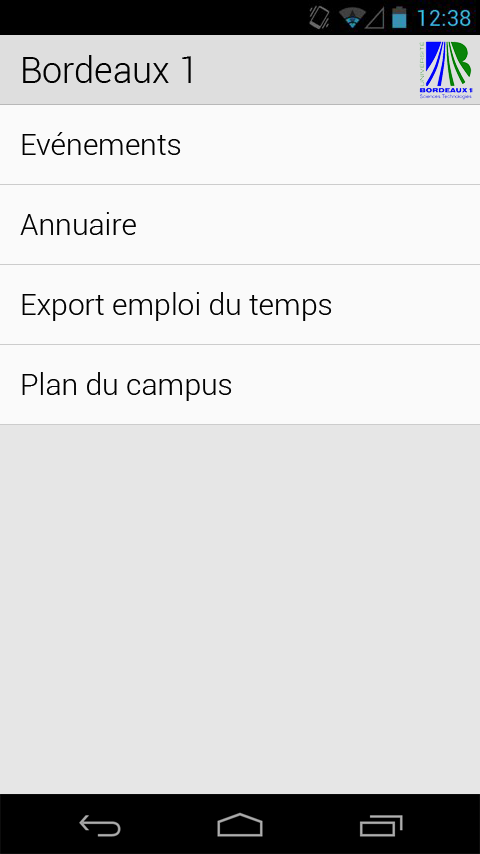
\includegraphics[width=0.8\textwidth]{resources/ui_preview/02}
    \caption{Vue d'accueil de l'application}
    \label{fig:02}
  \end{minipage}
  \hspace{-60pt}
\end{figure}


\begin{figure}
  \begin{minipage}[t]{8cm}
    \centering
    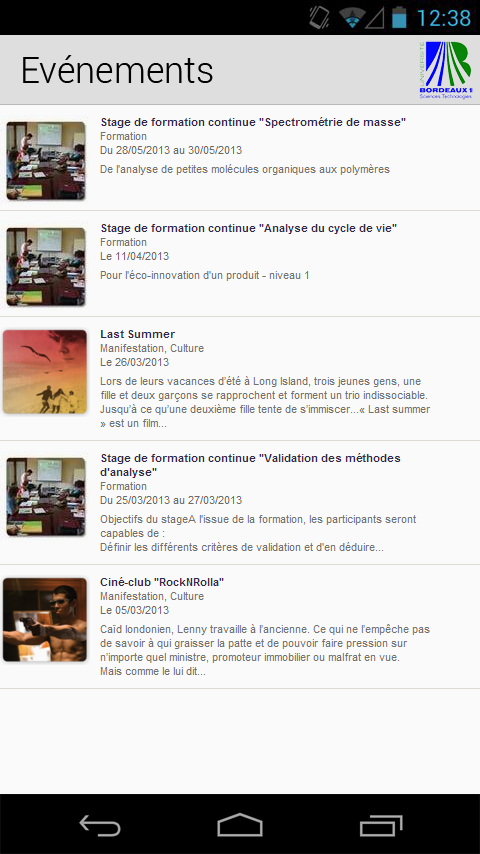
\includegraphics[width=0.8\textwidth]{resources/ui_preview/03}
    \caption{Vue des filtres des résultats en fonction des établissements préalablement choisis. Cette fonctionnalité est accessible en touchant le logo (situé en haut à gauche) de l'application uniquement depuis l'écran d'accueil.}
    \label{fig:03}
  \end{minipage}
  \hspace{+20pt}
  \begin{minipage}[t]{8cm}
    \centering
    
\includegraphics[width=0.8\textwidth]{resources/ui_preview/04}
    \caption{Vue des événements. Pour lire la news et arriver sur l'écran de la figure~\ref{fig:06}, il suffit d'appuyer sur la news correspondante. Par défaut, toutes les news sont affichées. On a également la possibilité de les afficher par catégories. La liste des catégories est disponible via la touche menu.}
    \label{fig:04}
  \end{minipage}
  \hspace{-60pt}
\end{figure}


\begin{figure}
  \begin{minipage}[t]{8cm}
    \centering
    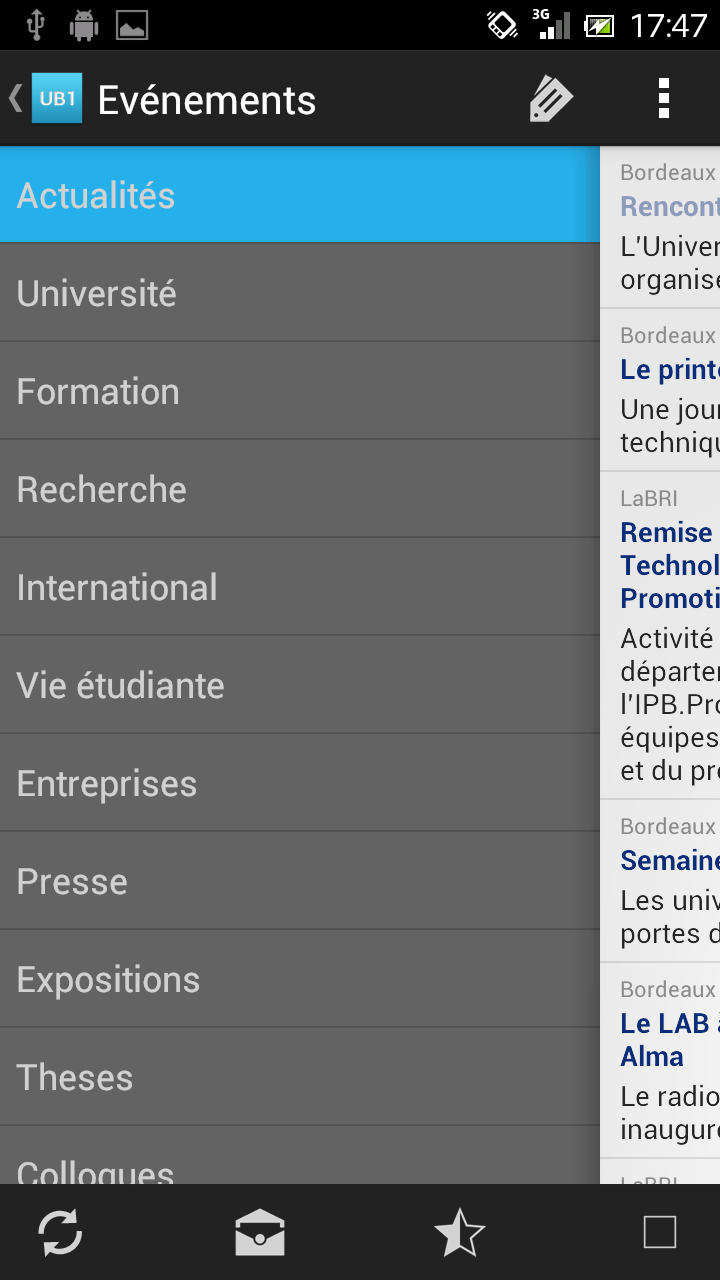
\includegraphics[width=0.8\textwidth]{resources/ui_preview/05}
    \caption{Liste des catégories pour afficher les news.}
    \label{fig:05}
  \end{minipage}
  \hspace{+20pt}
  \begin{minipage}[t]{8cm}
    \centering
    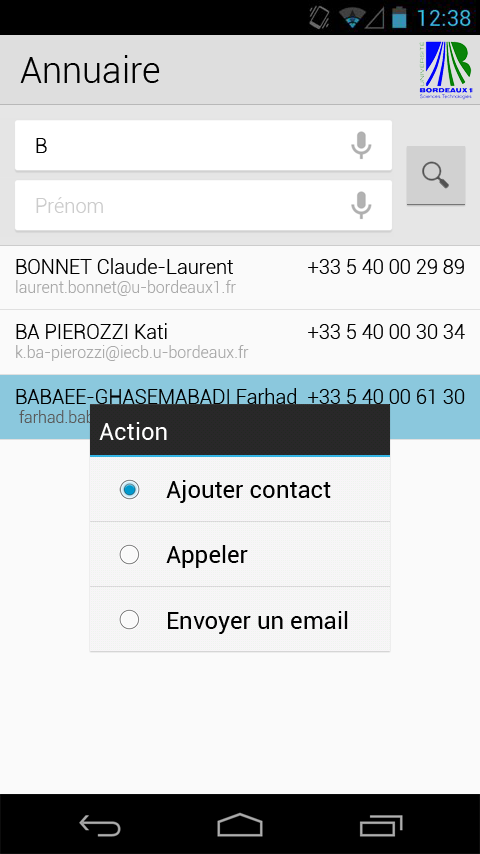
\includegraphics[width=0.8\textwidth]{resources/ui_preview/06}
    \caption{Vue détaillée d'une news. Le bouton ``plus'' situé en haut à droite permet d'ajouter l’événement au calendrier du smartphone.}
    \label{fig:06}
  \end{minipage}
  \hspace{-60pt}
\end{figure}


\begin{figure}
  \begin{minipage}[t]{8cm}
    \centering
    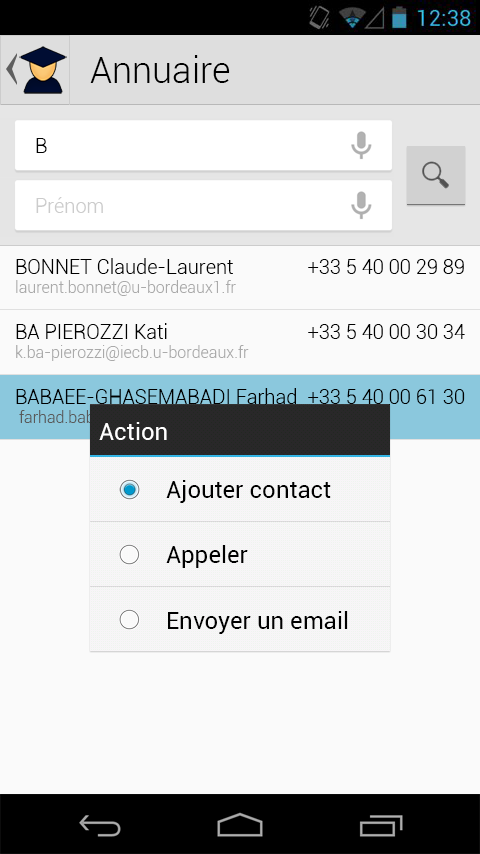
\includegraphics[width=0.8\textwidth]{resources/ui_preview/07}
    \caption{Vue de l'annuaire.}
    \label{fig:07}
  \end{minipage}
  \hspace{+20pt}
  \begin{minipage}[t]{8cm}
    \centering
    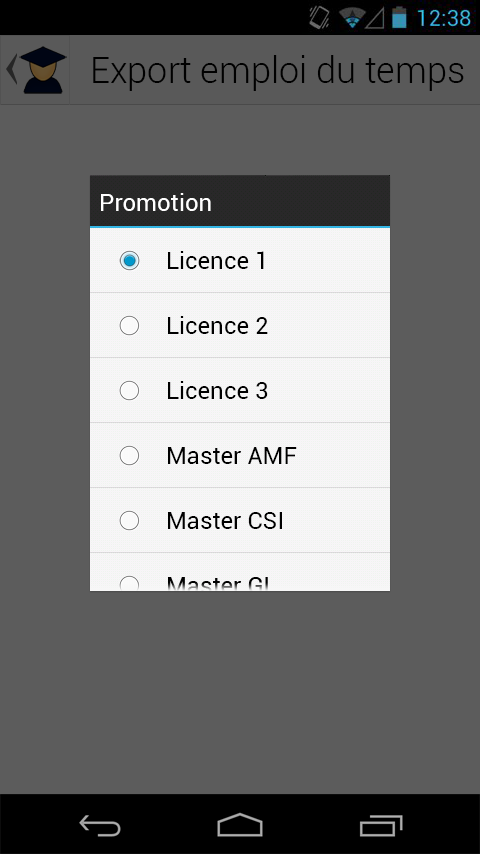
\includegraphics[width=0.8\textwidth]{resources/ui_preview/08}
    \caption{Vue des résultats de l'annuaire.}
    \label{fig:08}
  \end{minipage}
  \hspace{-60pt}
\end{figure}


\begin{figure}
  \begin{minipage}[t]{8cm}
    \centering
    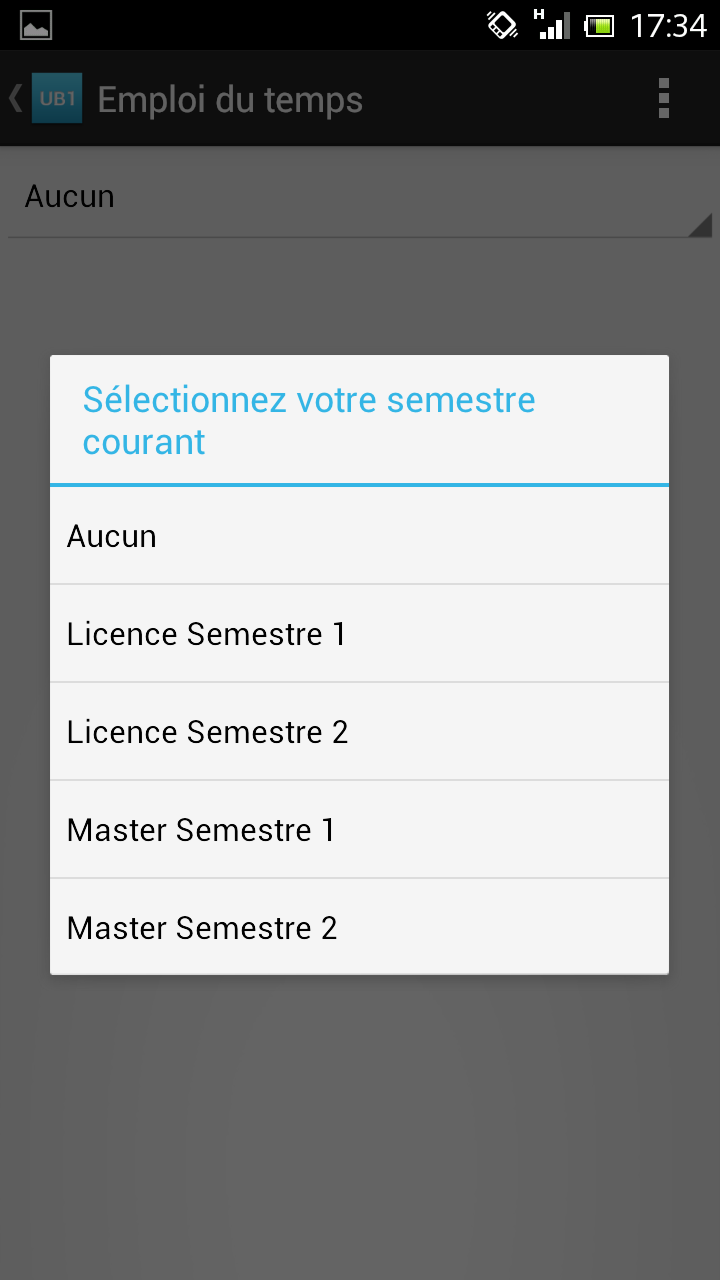
\includegraphics[width=0.8\textwidth]{resources/ui_preview/09}
    \caption{Export de l'emploi du temps. L'application demande la promotion seulement la première fois et il faudra aller dans les paramètres pour la modifier ultérieurement.}
    \label{fig:09}
  \end{minipage}
  \hspace{+20pt}
  \begin{minipage}[t]{8cm}
    \centering
    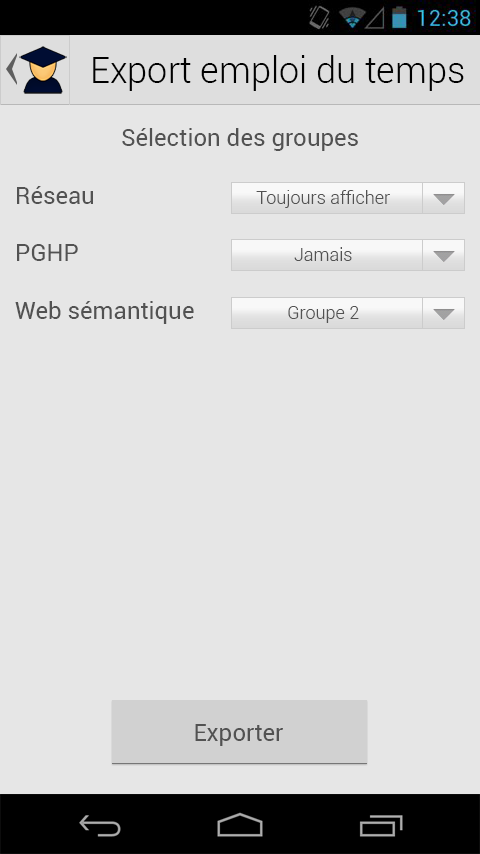
\includegraphics[width=0.8\textwidth]{resources/ui_preview/10}
    \caption{Sélection des groupes pour l'export de l'emploi du temps.}
    \label{fig:10}
  \end{minipage}
  \hspace{-60pt}
\end{figure}
\chapter{Gestion du projet}

\section{Outils de développement}
Dès le début de notre projet, nous avons décidé d’utiliser \emph{git} qui nous a paru être une solution plus complète comparée à \emph{svn}. Au fur et à mesure que nous pensions à une tâche à effectuer, ou que nous détections un bug à corriger, nous avons ajouté une \emph{issue} (problème ou tâche à effectuer) à notre projet sur GitHub. L’issue tracker de GitHub est très pratique, il permet de trier les issues par catégories, de les assigner à des membres du projet, ou encore d’ajouter des commentaires. De plus il suffit de préciser le numéro de l’issue que l’on corrige lors d’un commit pour fermer cette tâche automatiquement. Git offre également la possibilité de créer des branches qui permettent d’implémenter des fonctionnalités séparément, puis de fusionner les branches une fois terminée.

\section{Répartition des tâches}
Dans un premier temps, nous avons segmenté l’implémentation de notre projet en travaillant sur les deux fonctionnalités principales: la récupération des événements, et la recherche dans l’annuaire. \\
Etant donné que pour chacune de ces deux tâches, il fallait s’occuper séparément de la partie concernant l’Université de Bordeaux 1 et de celle concernant le LaBRI, quatre tâches distinctes étaient à notre disposition ce qui nous a permis de aisément répartir le travail entre les membres de l’équipe. Le fait que certaines de ces tâches ayant été plus simples à implémenter que d’autres, nous a permis d’avoir beaucoup d’interactions entre développeurs et donc beaucoup d’entraide.\\\\

Une fois que nous avons constaté que l’implémentation des fonctionnalités principales évoluait vite et qu’elle était quasiment finalisée , nous avons orienté deux membres de l’équipe pour s’intéresser aux fonctionnalités secondaires de notre application: l’accès aux emplois du temps, et le plan du campus. Là aussi avaient lieu beaucoup d'interactions dans l’équipe afin de pouvoir disposer de l’avis de plusieurs personnes lors de l’implémentation de certaines fonctionnalités.\\
Une fois les tâches secondaires finies, l’application était à un stade très avancé, tous les besoins fonctionnels  étaient achevés, il ne manquait alors plus que quelques touches de finalisation à apporter au sein des fonctionnalités principales. L’ensemble des membres de l’équipe ont alors pu contribuer à la mise au point finale.\\
La phase finale de test a alors commencé, au sein de laquelle la répartition des tests à effectuer a été faite en fonction des tâches que chacun des membres a effectuées.

\section{Tests Unitaires}
Afin de s'assurer que notre code soit robuste, nous avons effectué des tests unitaires, visant a s'assurer que toutes les parties de notre code fonctionnent correctement. Nous avons déterminé que les unités les plus petites de notre projet sont les classes; les tests unitaires portent donc sur ces éléments. Les classes les plus importantes de l’application sont les \emph{Activity}, car elles s’occupent du fonctionnement de chaque partie de l’application (événements, annuaire, ...). Il a donc fallu tester ces classes en priorité.\\

Pour cela, nous avons utiliser Robotium, un assistant open source pour l'élaboration de tests sous Android. Qui peut notamment simuler des clics sur l'écran, ainsi que tout autre geste nécéssaire pour tester une application Android.
Cet outil permet également de tester la couverture du code d'une application Android, mais les bibliotheques externes ont empeché Robotium de tester la couverture de notre application.
\chapter{Difficultés rencontrées}

Une des difficultés principales de ce projet tenait de l’apprentissage de l’API Android, et de son fonctionnement. L’API Android étant vaste, il n’était pas toujours facile de savoir si nous avions trouvé la solution optimale à un problème donné.\\
Nous avons décidé d'utiliser un \emph{ViewPager} afin de rendre le défilement d’un événement à un autre plus ergonomique. Or pour cela il a fallu implémenter une nouvelle activité. Ceci a légèrement compliqué l'enregistrement des événements comme lus depuis cette activité. Nous avons cherché la meilleure méthode de transmettre des données d’une activité à une autre, et sommes arrivés à la sérialisation d’objets à l'aide des objets de type \emph{Intent}. Cette méthode n'est pas forcément la solution idéale, mais semble être le moyen le plus apte à réaliser le travail nécessaire. \\

Lors de l’implémentation de l’extraction des dates, nous avons rencontré des problèmes concernant l’inclusion des librairies CUP et JFlex. Les méthodes n’étaient pas reconnues au sein du projet, rendant leur utilisation impossible.
Nous avons donc opté pour l'utilisation d'expressions régulières qui reconnaissent des dates. \\

En ce qui concerne les événements, nous avons dû faire comme prévu, deux récupérations d’information différentes, le parsing des flux RSS et le parsing des pages HTML.
Le parsing des flux et des pages a donné lieu à de nouvelles difficultés, notamment concernant les dates. Puisque beaucoup d'événements avaient la mauvaise date, voire même aucune date, nous avons dû essayer de déterminer la date correcte à partir du texte de l'événement. \\

Concernant les pages HTML, nous avons dû comprendre comment étaient organisées les pages, quels étaient les éléments à entrer dans la requête afin de récupérer les événements sur une certaine durée. Nous avons utilisé \emph{Jsoup} pour extraire les éléments. Ainsi, étant donné que les pages HTML du LaBRI sont agencées d'une certaine forme, il a fallu adapter le code pour parser ces pages.
Bien que la tâche ne nous fut pas incombée, nous voulions vérifier que les événements étaient complets, afin de ne pas encombrer l'application d'informations incompletes, voire inutilisables. En effet, certains d’eux ne possèdent pas de titre ou de descriptif, ou encore contiennent des informations inutilisables, voire insensées (voir exemple ci-dessous).

\begin{adjustbox}{minipage=1.0\textwidth, margin=0pt \smallskipamount, center}
\begin{lstlisting}[style=HTML, label=htmlCode, caption=Exemple d'événement HTML sans contenu (descriptif vide)]
<table width=100% cellspacing=0 style="border: solid 1px 
   #D3CFC4;">
   <tr>
      <td bgcolor="#c0c0">
         2013-03-21 <!--date-->
      </td>
      <td
         colspan=4 class="surligne">
         <b>
            RENCONTRE P UNG  <!-- titre -->
         </b>
      </td>
   </tr>
   <tr>
      <td width=100 valign=top>
         11:00-12:00        <!-- horaire -->
         <br>SALLE 1278     <!-- lieu -->
      </td>
      <td colspan=4 width=640>
         Intervenant: <br><br>
         <div align=justify>
         <!-- description -->
         </div>
      </td>
   </tr>
   <tr>
      <td></td>
      <td bgcolor=#cccccc width=75 align=center>
      <a href="javascript:openInfosActu('9121', '7371', 'groupe_details', '23', '0');">
         Plus d'infos</a>
      </td>
      <td width=435>&nbsp;<img src="../images/document.gif" title="Documentslies"></td>
</table>
\end{lstlisting}
\end{adjustbox}

\wl Nous avons eu des difficultés avec l’utilisation de \emph{ContentProvider} pour la gestion des événements du calendrier. En effet, selon les modèles de smartphone, l’utilisation de l’API est différente à cause notamment de la surcouche logicielle ajoutée par les constructeurs. Nous avons finalement décidé d’effectuer l’import de l’emploi du temps dans le calendrier par défaut. D’autres difficultés ont également été rencontrées pour insérer tous les événements en une fois (insertion par lots, ou \emph{batch insert}). Mais après plusieurs expérimentations, de multiples recherches et la lecture de nombreux posts sur l’excellent forum StackOverflow, nous sommes parvenu à implémenter cette fonctionnalité. \\

Nous avons également eu quelques soucis pour réceptionner les réponses des requêtes que nous soumettions auprès du serveur LDAP de Bordeaux 1. Le serveur refusait de donner suite aux requêtes renvoyant plus de dix résultats et nous affichait le message d'erreur \textit{size limit exceeded (maximum size is 10)}. C'est donc une restriction imposée par le serveur et il fallait faire avec. Cependant, il fallait tout de même trouver un système pour limiter la taille de nos requêtes à dix éléments pour éviter de lever une \textit{LDAPException} qui nous empêchait d'accéder aux dix premiers contacts retournés. Une recherche plus approfondie au sein de la documentation de la SDK \textit{UnboundID} nous a permis de trouver la solution au problème. \\ 

\begin{figure}[h!]
  \label{fig:simple_paged_results}
  \center
  \setlength\fboxsep{5pt}
  \setlength\fboxrule{0.5pt}
  \fbox{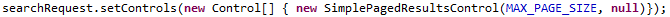
\includegraphics[width=1.0\textwidth]{resources/simplePagedResults.png}}
\end{figure}


L'utilisation du système \emph{Simple paged result control} propre au protocole LDAP nous a permis de demander au serveur de nous renvoyer une seule page de taille \textit{MAX\_PAGE\_SIZE=10} contenant les dix premiers résultats de la requête. Si la recherche effectuée contient donc plus de dix résultats, il seront ignorés à cause des restrictions techniques propres au serveur LDAP en question.
\chapter{Extensions et améliorations possibles}
Il existe un grand nombre d’améliorations envisageables pour notre application qui est censée évoluer constamment après son déploiement.
Dans un premier temps, il faudrait ajouter le support pour d’autres éventuels établissements appartenant au campus tels que l’IUT de Bordeaux 1 ou l’INRIA. 
Il est alors à prévoir qu’on risque très probablement d’avoir d’autres pages HTML organisées différemment à parser, et donc de nouveaux modules à intégrer.\\\\
 
Lorsqu’on a commencé à implémenter l’annuaire, notre choix initial était d’utiliser le serveur LDAP de l’Université de Bordeaux 1 ainsi que celui du LaBRI pour accéder aux contacts des établissements en question. Le problème étant que le serveur LDAP du LaBRI n’est pas accessible depuis l’extérieur sans authentification, il ne nous restait pas d’autre choix que de parser la page HTML du LaBRI en question. Une éventuelle amélioration possible aurait alors été d’utiliser le serveur LDAP sécurisé et de demander à l’utilisateur de s’authentifier s'il veut effectuer une recherche de contacts au sein du LaBRI. Cela aurait nettement amélioré le temps de recherche dans l’annuaire. Mais dans le cas pratique, l’utilisateur perdrait énormément de temps à entrer ses identifiants afin de lancer la recherche et accéderait finalement encore moins vite aux contacts qu’avec notre implémentation actuelle. Cette amélioration est donc à voir uniquement d’un point de vue d’optimisation des  performances de l’application, et non du côté facilité d’utilisation.\\\\

Pour le plan du campus, on pourrait également donner plus de détails concernant les marqueurs en donnant plus d’informations concernant celui-ci. Par exemple pour les bâtiments, on pourrait proposer à l’utilisateur de consulter le plan intérieur du bâtiment en question, ou pour les restaurants d’afficher les horaires d’ouverture et de fermeture ainsi que leur numéro de téléphone.\\
Une autre extension possible serait de pouvoir calculer les itinéraires routiers à pied ou en voiture afin de faciliter l’accès au campus, et à ses différents bâtiments. Il serait alors possible d’indiquer à l’utilisateur le chemin à effectuer pour se rendre à pied d’un bâtiment du campus à un autre.\\
Nous avons également réfléchi à une amélioration de l’outil de recherche intégré, qui serait capable de nous proposer dynamiquement une liste de suggestions correspondant à notre recherche en proposant un service d'auto-complétion.\\\\

En ce qui concerne l’emploi du temps, une fonctionnalité qui aurait pu accélérer l’affichage de l’emploi du temps ainsi que de l’améliorer esthétiquement aurait été de créer nous-même une vue de l’emploi du temps au sein de l’application en récupérant les informations nécessaires, et donc ne pas avoir à rediriger l’utilisateur vers le navigateur Internet qui prend du temps à s’ouvrir ainsi qu’à afficher les emplois du temps en format HTML. On pourra aussi sauvegarder les choix de l'utilisateur pour lui donner un accès rapide à son emploi du temps du semestre courant.\\
\chapter{Annexe}

\begin{figure}[h!]
  \label{fig:method_prof1}
  \center
  \setlength\fboxsep{5pt}
  \setlength\fboxrule{0.5pt}
  \fbox{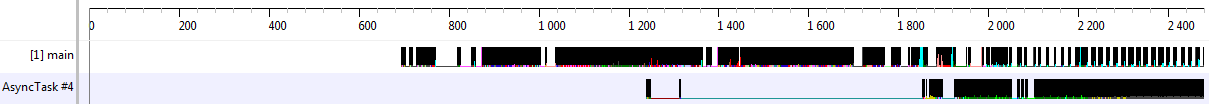
\includegraphics[width=0.9\textwidth]{resources/profiling/method_profiling/Bordeaux1_events.png}}
  \caption{Method profiling montrant le temps nécessaire à parser les événements de Bordeaux 1}
\end{figure}

\begin{figure}[h!]
  \label{fig:method_prof2}
  \center
  \setlength\fboxsep{5pt}
  \setlength\fboxrule{0.5pt}
  \fbox{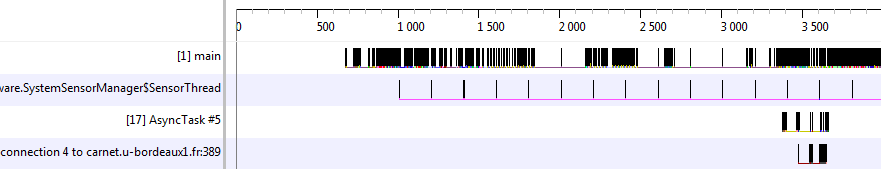
\includegraphics[width=0.9\textwidth]{resources/profiling/method_profiling/Bordeaux1_directory.png}}
  \caption{Method profiling montrant le temps nécessaire pour récupérer les résultats d'une requête auprès du serveur LDAP de Bordeaux 1}
\end{figure}

\begin{figure}[h!]
  \label{fig:method_prof3}
  \center
  \setlength\fboxsep{5pt}
  \setlength\fboxrule{0.5pt}
  \fbox{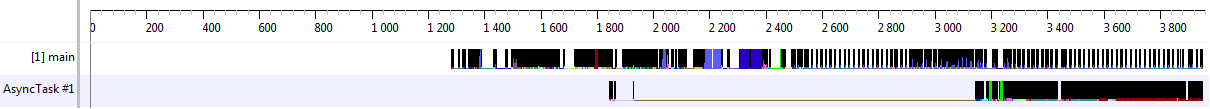
\includegraphics[width=0.9\textwidth]{resources/profiling/method_profiling/Labri_events.png}}
  \caption{Method profiling montrant le temps nécessaire à parser les événements du LaBRI}
\end{figure}

\begin{figure}[h!]
  \label{fig:method_prof4}
  \center
  \setlength\fboxsep{5pt}
  \setlength\fboxrule{0.5pt}
  \fbox{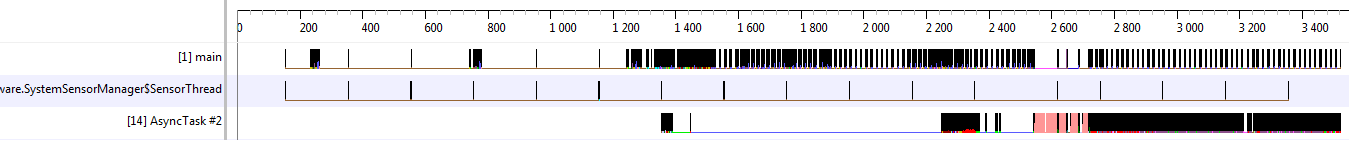
\includegraphics[width=0.9\textwidth]{resources/profiling/method_profiling/Labri_directory.png}}
  \caption{Method profiling montrant le temps nécessaire à parser les contacts du LaBRI}
\end{figure}

\nocite{*}
\bibliographystyle{unsrt}
\bibliography{biblio}

\end{document}
 
